

For the programming elements of the game, a bespoke language called CatCode was created. This language would be designed to control entities in game, and was never intended to be fully featured. Early on, in requirement production period, it was decided that the editor, runner and output devices should be interchangeable to reduce coupling and increase flexibility. The relationships are shown in \autoref{fig:design/CatCodeBack/Overview}. This meant that CatCode could be initially developed as a text-based language with Graphical CatCode implemented at a later date. This also meant that CatCode could control entities other than \textit{CatBot}.

This system ended up far more complicated than anticipated and was largely responsible for the long Core System development time. A lot of the complexity was not originally anticipated, even with period dedicated to design, because many of the components, such as \textit{CatThreads}, had to be added due to unforeseen complications.

\begin{figure}[h]
    \centering
    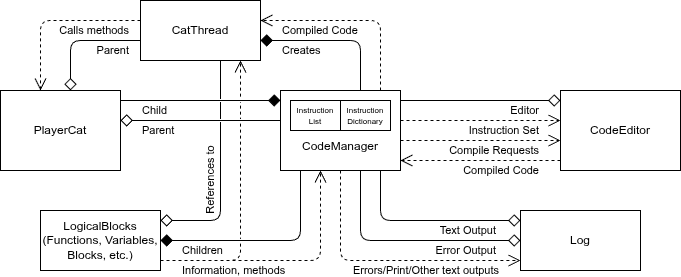
\includegraphics[width=1\linewidth]{C5/CatCode/catCodeOverview.png}
    \caption{CatCode overview class diagram}
    \label{fig:design/CatCodeBack/Overview}
\end{figure}

\subsection{Components}

As shown in \autoref{fig:design/CatCodeBack/Overview}, there are multiple main components, whose responsibilities are listed in \autoref{tab:design/CatCode/ComponentResponsibilities}. The centre, and manager of this system is the \textit{CatCodeManager} (sometimes semantically the \textit{CodeManager}, \texttt{res://src/catCode/cat\_code\_ manager.tscn}). This is instanced as a child of the node it is controlling. It stores the \textbf{InstructionSet}, a pair of variables: \texttt{instruction\_list} (a list of references instruction blocks) and \texttt{instruction\_dict} (a dictionary of the same references). By default, the \textit{LogicBlock} nodes are instanced as shildren of the \textit{CodeManager} node. Refer to \autoref{fig:catCodeSpec/files} for the file locations.

\begin{fullwidthtable}[]
    \centering
    \begin{tabular}{llp{10cm}}\toprule
        Node(s)	& Variable & Responsibilities \\\midrule
        <Entity> & \texttt{parent} & Executes movement functions such as \texttt{jump()}. \\
        \textit{CodeManager} & \texttt{this} & Creates and manages \textit{CatThreads} to run the code. Constructs and stores the instruction set. \\
        \textit{CatThread} & \texttt{threads[]} & Run the code, calling functions of \texttt{parent} where required. \\
        \textit{CodeEditor} & \texttt{editor} & Edits and compiles the code. \\
        \textit{Log} & \texttt{text\_output} & Handles text outputs, implementing method \texttt{print\_line(message)}. \\
        \textit{ErrorLog} & \texttt{error\_output} & Outputs error messages, if unassigned, this will be handled by the logger. \\
        \textit{StabilityTarget} & \texttt{stability\_target} & The entity that will be damaged by errors. \\
        \textit{InstructionSource} & \texttt{instruction\_source} & The children of this node are used to compile the instruction set. By default, it will be the \textit{CodeManager}. \\
        \textit{LogicBlocks} & N/A & Stores both the metadata and methods for a block. \\ \bottomrule
    \end{tabular}
    \caption{CatCode components and their responsibilities}
    \label{tab:design/CatCode/ComponentResponsibilities}
\end{fullwidthtable}

\subsection{The Logic Block Family of Classes}

The \texttt{logic\_block} family of classes, sometimes semantically called \textit{LogicalBlocks}, handle the back-end functionality of the blocks. These store the metadata and implementation of the function that of CatCode blocks. There are multiple different types of blocks, explained below and in the class diagram in \autoref{fig:design/CatCode/LogicBlockClassDiagram}. Godot does have interfaces, instead abstract classes had to be used, nor does it support multiple inheritance, which greatly influenced this class structure.

\begin{fullwidthfigure}[h]
    \centering
    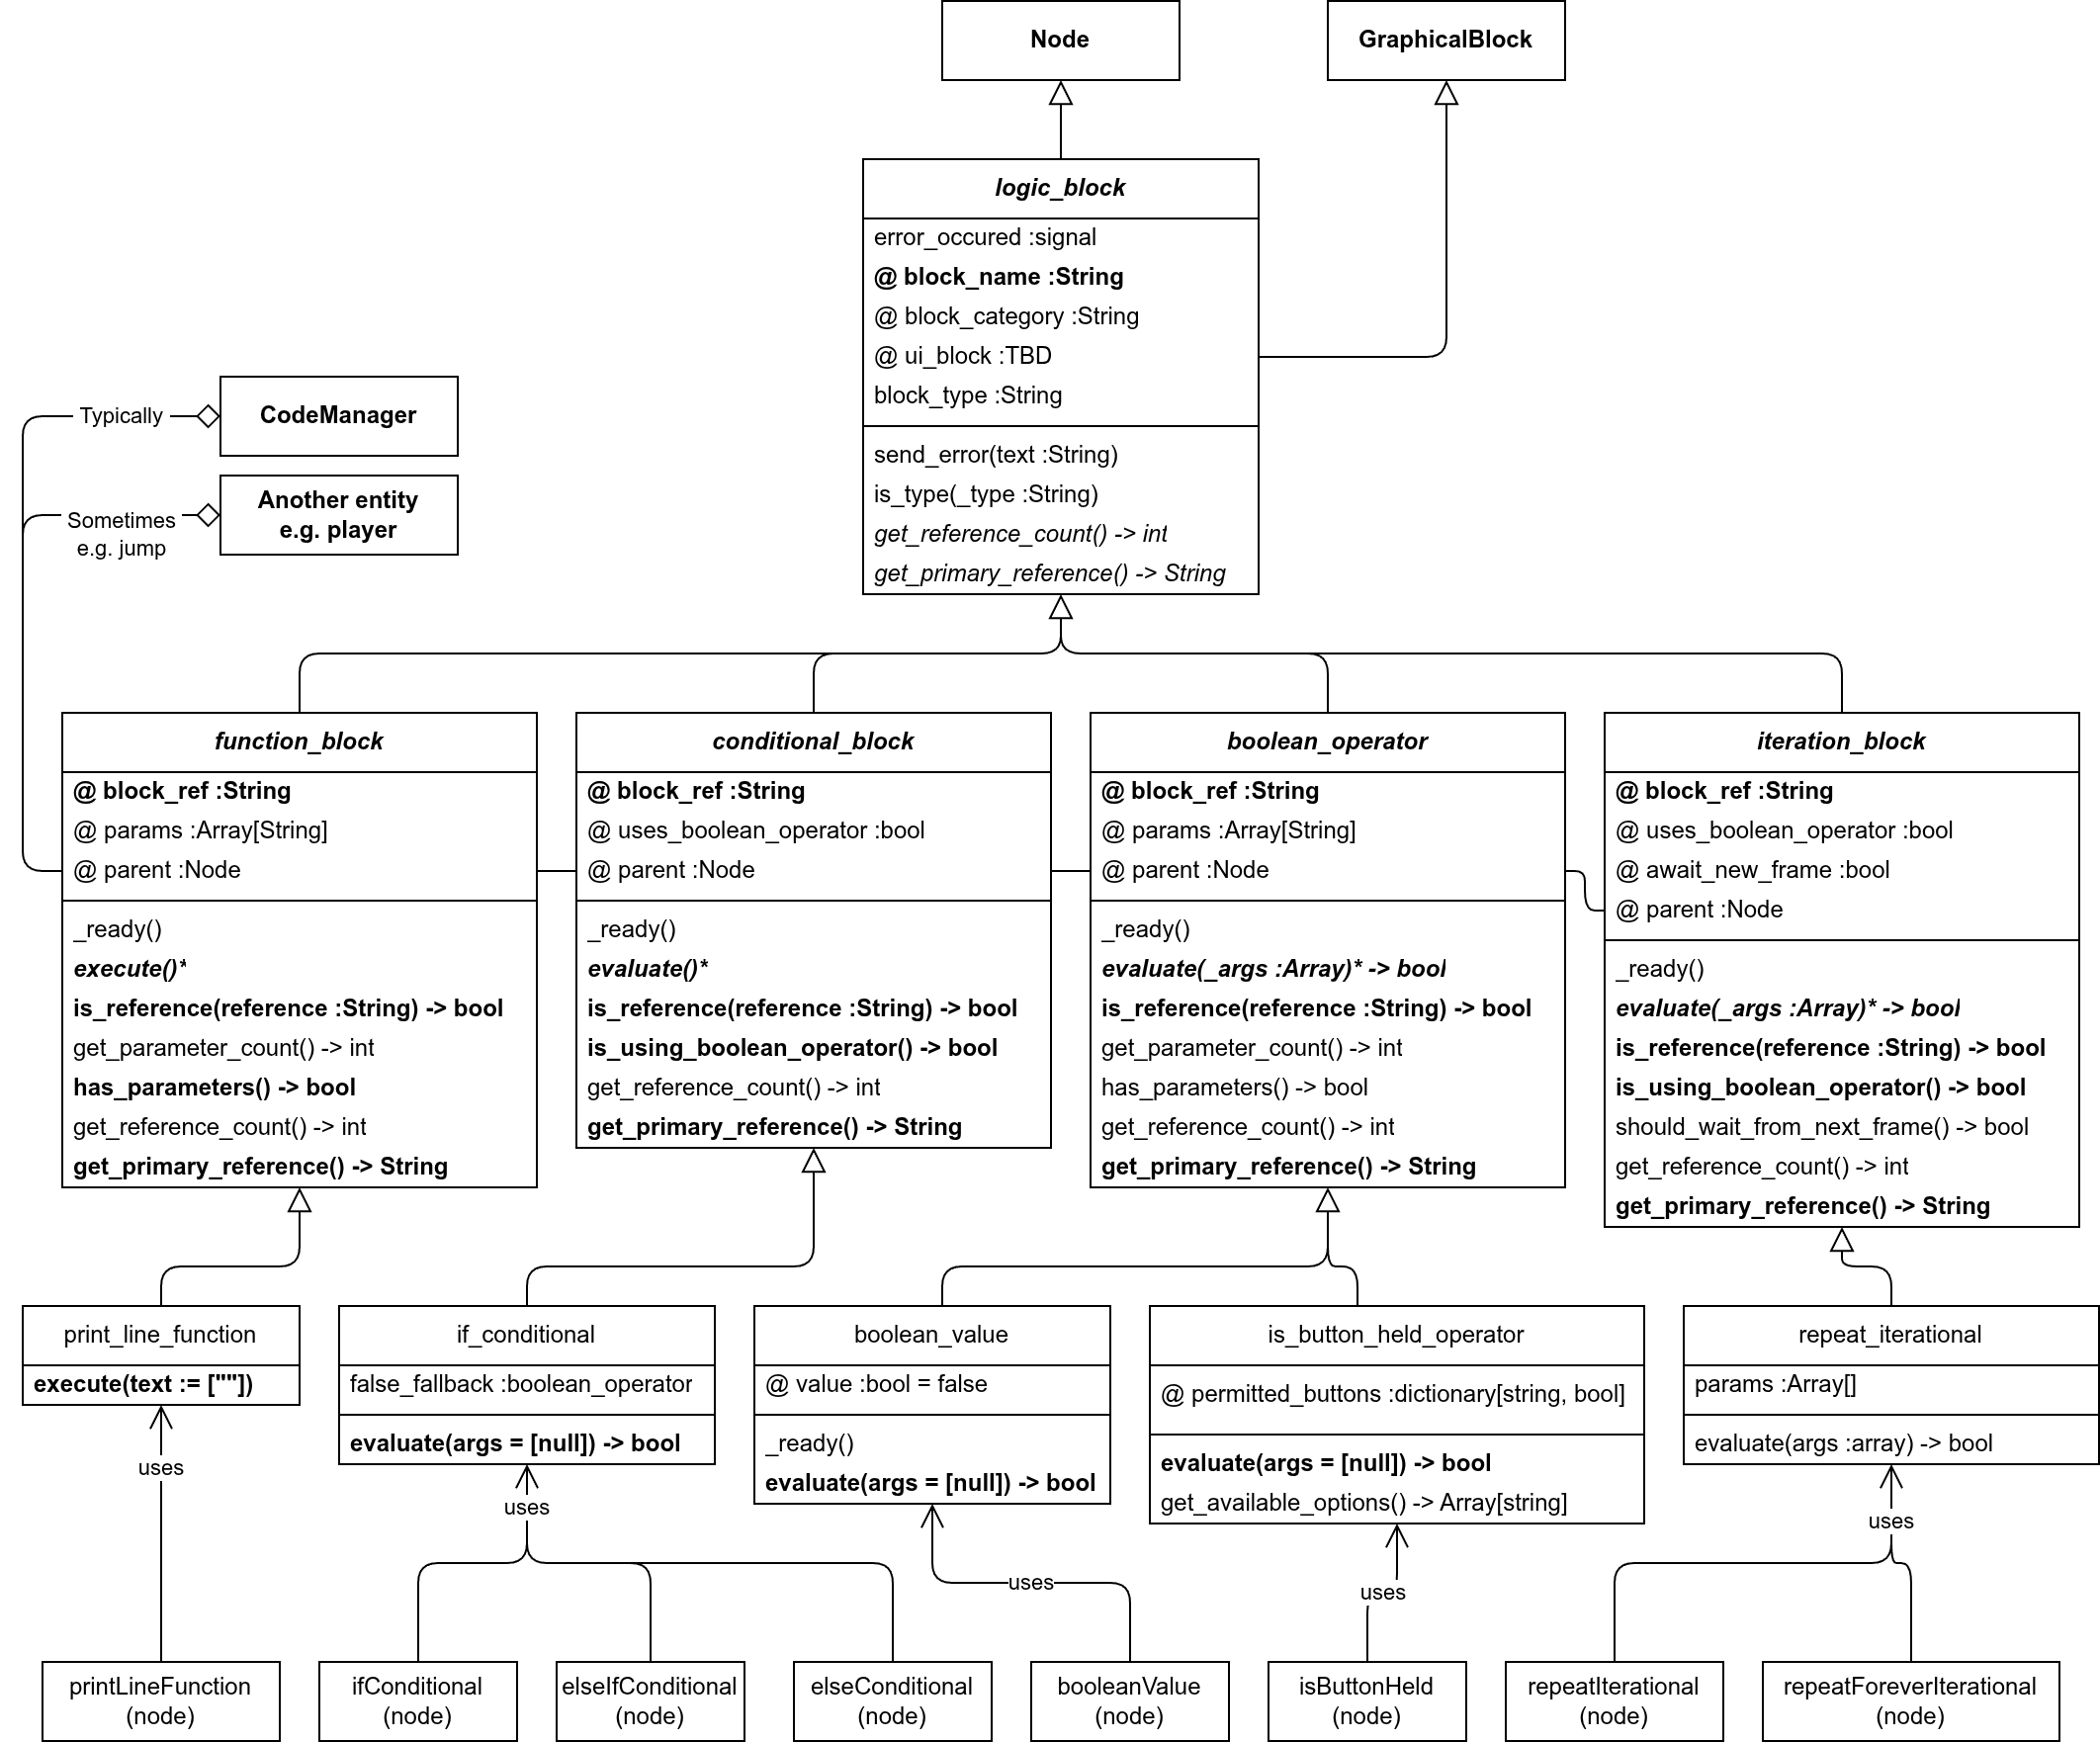
\includegraphics[width=1\linewidth]{C5/CatCode/catCode-LogicalBlocks-ClassDiagram.png}
    \caption{Partial class diagram of the LogicBlock family of classes}
    \label{fig:design/CatCode/LogicBlockClassDiagram}
\end{fullwidthfigure}

The \texttt{logicBlock} directory is separated into two folders: \texttt{nodes} and \texttt{scripts}, with the superclasses getting stored in \texttt{classes}, refer to \autoref{fig:catCodeSpec/files} to more detail on the locations. This was to aid with dragging and dropping nodes in the editor to add blocks to the instruction set as accidentally dropping a script file onto the \textit{CodeManager} rather than the node will override the \textit{CodeManager}'s script.

Whilst many nodes have their own final script, this is not required as most of the metadata for each block is stored using \texttt{@export} variables (which can be set for each node in the editor). The purpose of each superclass is available in TAB. \autoref{app:supp} contains the \nameref{app:supp} which details each of the blocks in full.

\textbf{TODO: Once words available are known}

\subsection{Constructing the Instruction Set}

\begin{figure}
    \centering
    \begin{subfigure}[t]{0.4\linewidth}
        \centering
        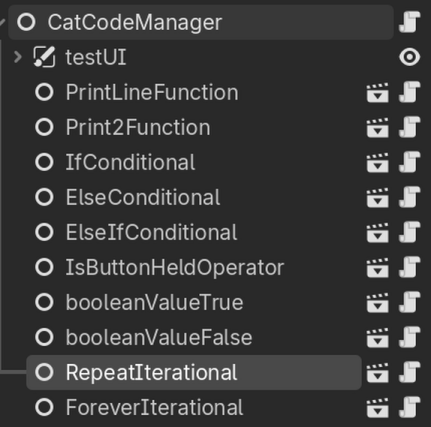
\includegraphics[height=1\linewidth]{C5/CatCode/ExampleCodeManager.png}
        \caption{CatCodeManager Instance}
    \end{subfigure}
    \begin{subfigure}[t]{0.4\linewidth}
        \centering
        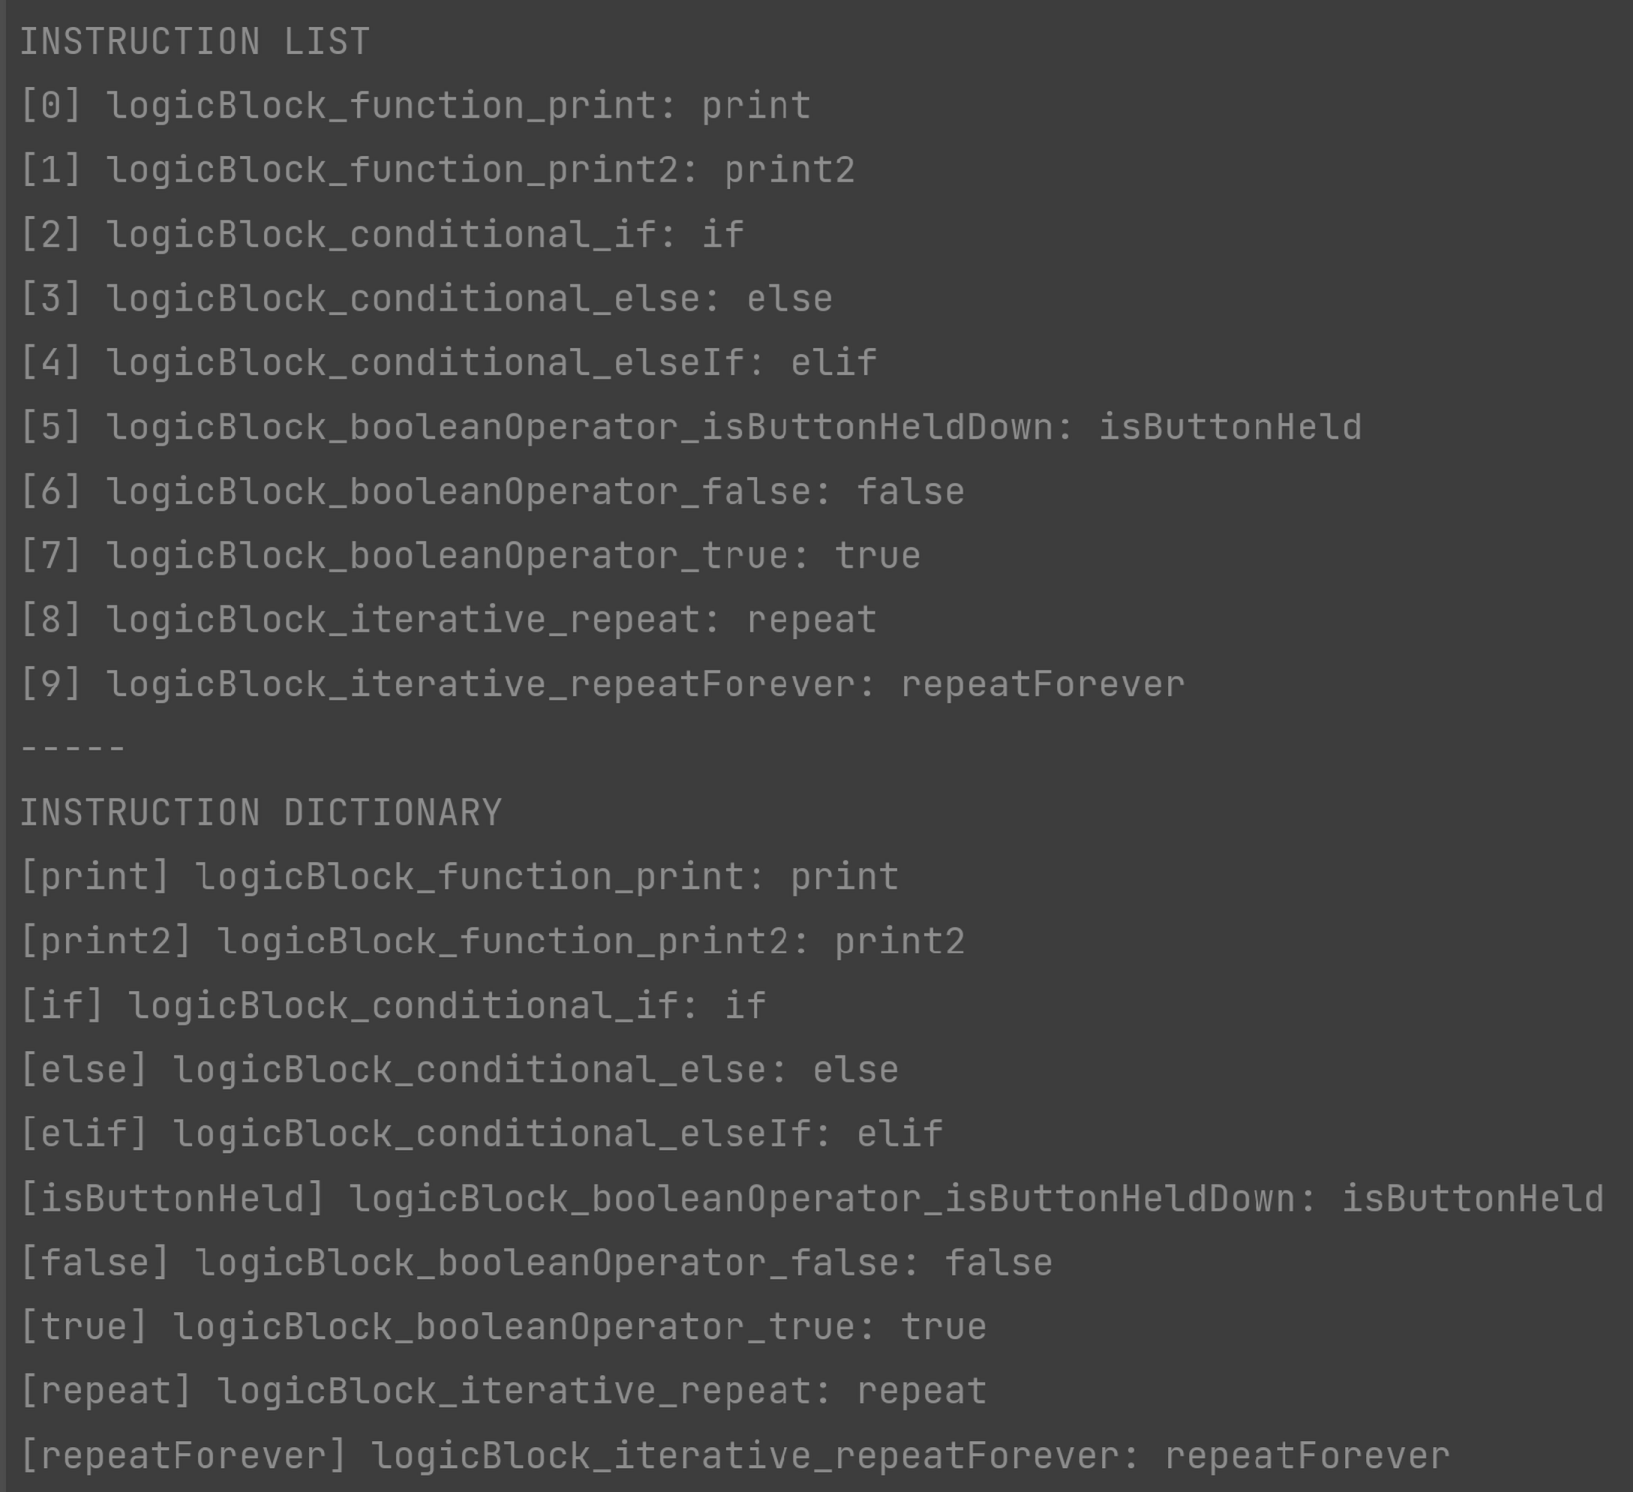
\includegraphics[height=1\linewidth]{C5//CatCode/instructionSetAndDictExamples.png}
        \caption{Resultant instruction set}
    \end{subfigure}
    \caption{Example CatCodeManager instance alongside its instruction set values}
    \label{fig:design/CatCode/ExampleCodeManagerInstance}
\end{figure}

The instruction set, for the level designer, is defined by dragging and dropping \textit{LogicBlock} nodes from the exploring onto the \textit{codeManager} node. Example shown in \autoref{fig:design/CatCode/ExampleCodeManagerInstance}. Certain nodes may require configuration within the inspector. When the \textit{codeManager} is instantiated, the \texttt{update\_instructions()} is called which creates the \texttt{instruction\_list} and \texttt{instruction\_dict}.

The \texttt{update\_instructions()} function does the following:

\begin{enumerate}
    \item Adds references to each of the child nodes from \texttt{instruction\_source} that are logic blocks to the list \texttt{instruction\_list}.\footnote{These nodes are identified through name (due to the lack of applicable universal \texttt{type()} method), taking advantage of the the naming scheme, \texttt{logicalBlock\_<type>\_<name>}, for logic blocks.}
    
    \item Iterates across this list, adding each block to the dictionary \texttt{instruction\_dict} where the key is the block's \texttt{block\_ref} and the value is a reference to the block.

    \item Emits the signal \texttt{instructions\_updated(new\_list :Array[logic\_block], new\_dict :Dictionary[String, logic\_block])}, to allow any relevant nodes to receive this new instruction set.
\end{enumerate}

\subsection{Compiled CatCode}

CatCode is compiled language. This is because, in many scenarios, a script is getting executed every frame meaning that execution speed is worth the cost in memory intensity. Because it is executed every frame, executions will greatly outnumber compilations. Also, relying on compiled CatCode for execution allowed the Code Editor to be swapped. It is the responsibility of the Code Editor to compile CatCode.

Compiled CatCode consists of an array of \texttt{instruction\_line} class instances (full definition available in \autoref{fig:design/CatCodeBack/instructionLineFull}). Each element represents a single line storing -- through \texttt{instruction\_line} -- a line's indent, a reference to the line's \textit{LogicBlock}, and its parameters. For interpretation to work as intended, the final block must be a \textit{pass} block where it's \texttt{indent} is \texttt{0}.


\begin{fullwidthfigure}
    \centering
    \begin{tcolorbox}[boxrule=0.25mm]
    \begin{verbatim}
class_name instruction_line

var indent :int
var primary_block :logic_block
var parameters :Array
var executable_function :bool = false
var iterative_element :bool = false
var selective_element :bool = false

func _init(_indent :int, _primary_block :logic_block, _parameters :Array = []):
    indent = _indent
    primary_block = _primary_block
    parameters = _parameters

    match primary_block.block_type:
        "function_block":
            executable_function = true
        "conditional_block":
            selective_element = true
        "iterative_block":
            iterative_element = true


func is_executable_function():
    return executable_function

func is_iterative_element():
    return iterative_element

func is_selective_element():
    return selective_element

func valid_parameters():
    return (primary_block.get_parameter_count() == len(parameters))

func uses_parameters():
    return primary_block.has_parameters()

func _to_string() -> String:
    return str(indent) + ": " + str(primary_block.block_name) + [...]
        "(" + str(parameters) + ")"

func get_next_indent() -> int:
    if iterative_element or selective_element:
        return indent + 1
    else:
        return indent
    \end{verbatim}
    \end{tcolorbox}
    \caption{Instruction class definition}
    \label{fig:design/CatCodeBack/instructionLineFull}
\end{fullwidthfigure}

\begin{fullwidthfigure}[h]
    \centering
    \begin{subfigure}[T]{0.415\linewidth}
        \centering 
        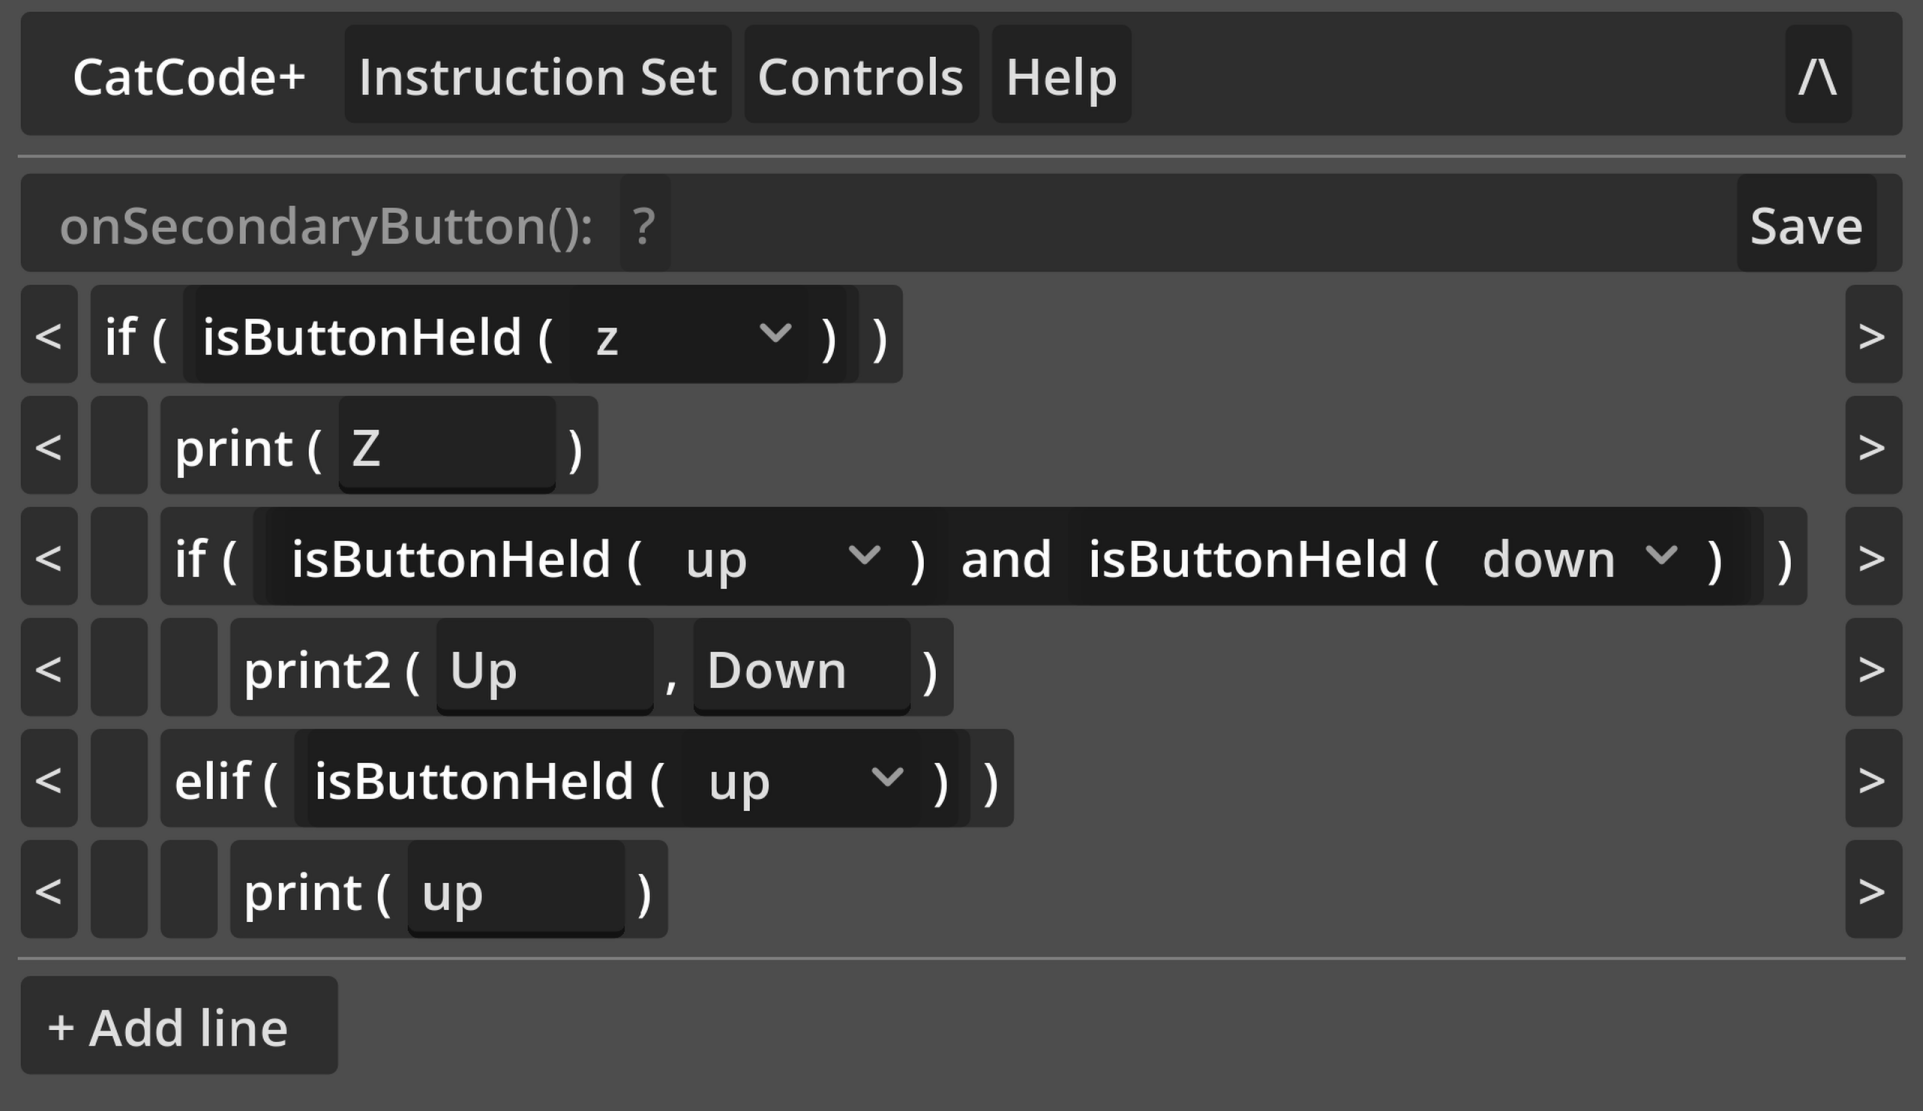
\includegraphics[width=1\linewidth]{C5//CatCode/CatCodeExample2.png}
        \caption{Uncompiled graphical CatCode}
    \end{subfigure}
    \begin{subfigure}[T]{0.5\linewidth}
        \begin{tabular}{lll}\toprule
            Ind. & Block & Parameters \\\midrule
            0 & \textit{if} & [\textit{isButtonHeld}, ["Z"]] \\
            1 & \textit{print} & ["Z"] \\
            1 & \textit{if} & [\textit{and}, [\textit{isBu...}, "up"], [\textit{isBu...}, "down"]] \\
            2 & \textit{print2} & ["Up", "Down"] \\
            1 & \textit{elif} & [\textit{isButtonHelf}, ["x"]] \\
            1 & \textit{print} & ["up"] \\
            0 & \textit{pass} & [] \\ \bottomrule
        \end{tabular}
        \caption{Compiled code, stored in array \texttt{compiled\_code}}
    \end{subfigure}
    \caption{Compiled CatCode example}
    \label{fig:placeholder}
\end{fullwidthfigure}

\subsection{Interpreting Compiled Code}

\textbf{TODO}